\chapter{Visão geral dos subsistemas}

%Devido a divisão do projeto nos subsistemas de tração, energia e estrutura;
%perfuração e coleta; localização no ambiente e infomações é necessário que haja uma proposta de
%integração dessas partes. Nessa proposta vamos tratar tração, energia e estrutura como módulo 1
%perfuração e coleta como módulo 2 e localização no ambiente e informações como módulo 3.
%Fica evidente, pelo curto tempo disponível, que os módulos devem começar a ser desenvolvidos simultaneamente.
%Porem, mais do que isso, é importante sincronizar atividades críticas e interdependentes tendo em vista a estrutura analítica
%do projeto.
%
%O módulo 1 alimenta o sistema como um todo e também recebe sinais de controle do módulo 3. Esses sinais são adquiridos
%pelos sensores de localização durante a rotina movimentação. Durante a rotina de perfuração o módulo 2 recebe sinais de
%de controle do módulo 3 e devolve o dado recolhido pelo sensor de umidade.
%
%Tendo em vista essa correlação, para que possamos realizar testes durante o desenvolvimento do projeto, os módulos 1 e 3
%devem manter ritimos proporcionais de progresso. O módulo 2 não retem outras atividades, já que só recebe dois tipos
%de sinal de controle e devolve a medição do sensor.

Com base nas discussões e propostas de solução iniciais,
formulou-se um esquemático capaz de descrever o sistema
eletrônico a nível modular. Este é composto por 5 módulos
distintos que visam a execução de atividades elementares
de modo a garantir a funcionalidade do sistema.
Atividades que, por sua vez foram definidas com base nos
requisitos levantados. A figura \ref{fig:visao_geral} ilustra esse esquemático.

\begin{figure}[!htbp]
\begin{center}
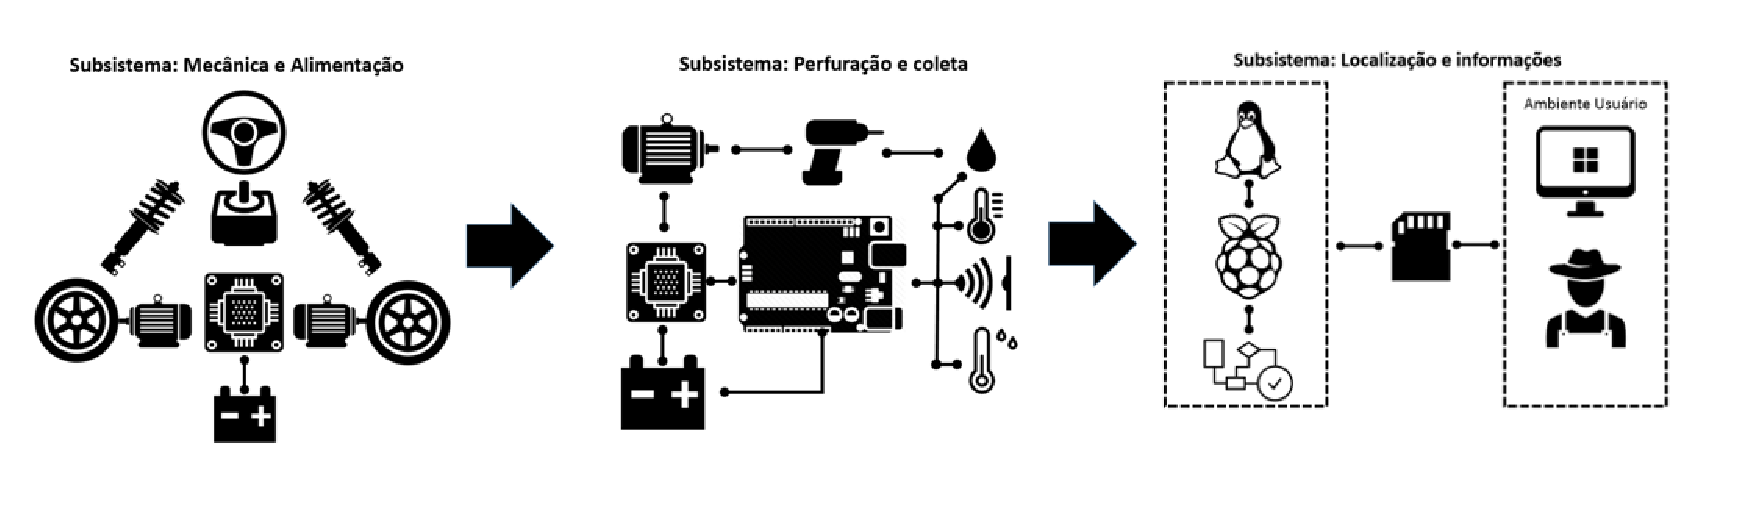
\includegraphics[width=.8\textwidth]{figuras/visao_geral.eps}
\caption{\label{fig:visao_geral}Visão geral do sistema.}
\end{center}
\end{figure}

\begin{description}
\item[Módulo de sensoriamento:] Responsável pela aquisição dos dados relativos à
umidade relativa e temperatura do ar, umidade relativa do solo e distância
entre o veículo e seu objeto de medição.
\item[Módulo de controle:] O módulo de controle destina-se primeiramente à
realização de leitura e envio de dados adquiridos a partir dos sensores
para a unidade de processamento. Além disso, destina-se a realizar o
controle dos atuadores com base nas informações recebidas pela unidade de processamento após o tratamento de dados.
\item[Unidade de processamento:] Destina-se ao tratamento dos dados
adquiridos pelos sensores de distância. Esse tratamento está relacionado
fundamentalmente ao grau de autonomia do veículo, visto que é necessária
alguma forma de mapear o ambiente, sendo assim será utilizado um sistema
operacional baseado em uma versão Linux embarcada para implementação
dos algoritmos de localização.
\item[Módulo de armazenamento:] Destina-se ao armazenamento dos dados
adquiridos ao longo do caminho. Este módulo mantém uma estreita relação
com a unidade de processamento, visto que trabalharão de forma conjunta
nas atividades de armazenamento.
\item[Módulo de Atuação:] Responsável pela atuação do sistema, ou seja,
a interação física com o ambiente também físico. Mais especificamente
o módulo destina-se à duas atividades; são elas a locomoção do veículo
e perfuração da terra. Os motores para o módulo já foram definidos
anteriormente no relatório.
\end{description}

\section{Arquitetura dos sistemas}
A arquitetura definida para o sistema a princípio foi definida pensando-se em um sistema a parte onde o usuário poderá acessar a partir da sua máquina um sistema web. Neste sistema, o usuário ou produtor, irá acessá-lo e entrará com informações a respeito de sua plantação, como comprimento do camalhão e quantidade de camalhões para que seja possível o robô obtenha os dados da plantação a ser percorrida.

Os dados referente aos camalhões da plantação serão passadas para o robô por um arquivo, como já dito antes, no formato csv. Uma vez que estes dados estejam no robô, eles serão tratados no módulo Plano. Este módulo é responsável pela inteligência do robô onde é definida a trajetória e pesa os critérios de decisão a ser tomada pelo robô. O módulo chamado Model será responsável de trazer e armazenar os dados em um banco de dados no robô. Já o módulo Atuador se comunica com os motores e realiza o movimento além de cuidar do sensoriamento. A seguir na figura \ref{fig:arquitetura_sistema}, temos em alto nível o modelo de arquitetura definido.

\begin{figure}[!htbp]
	\begin{center}
		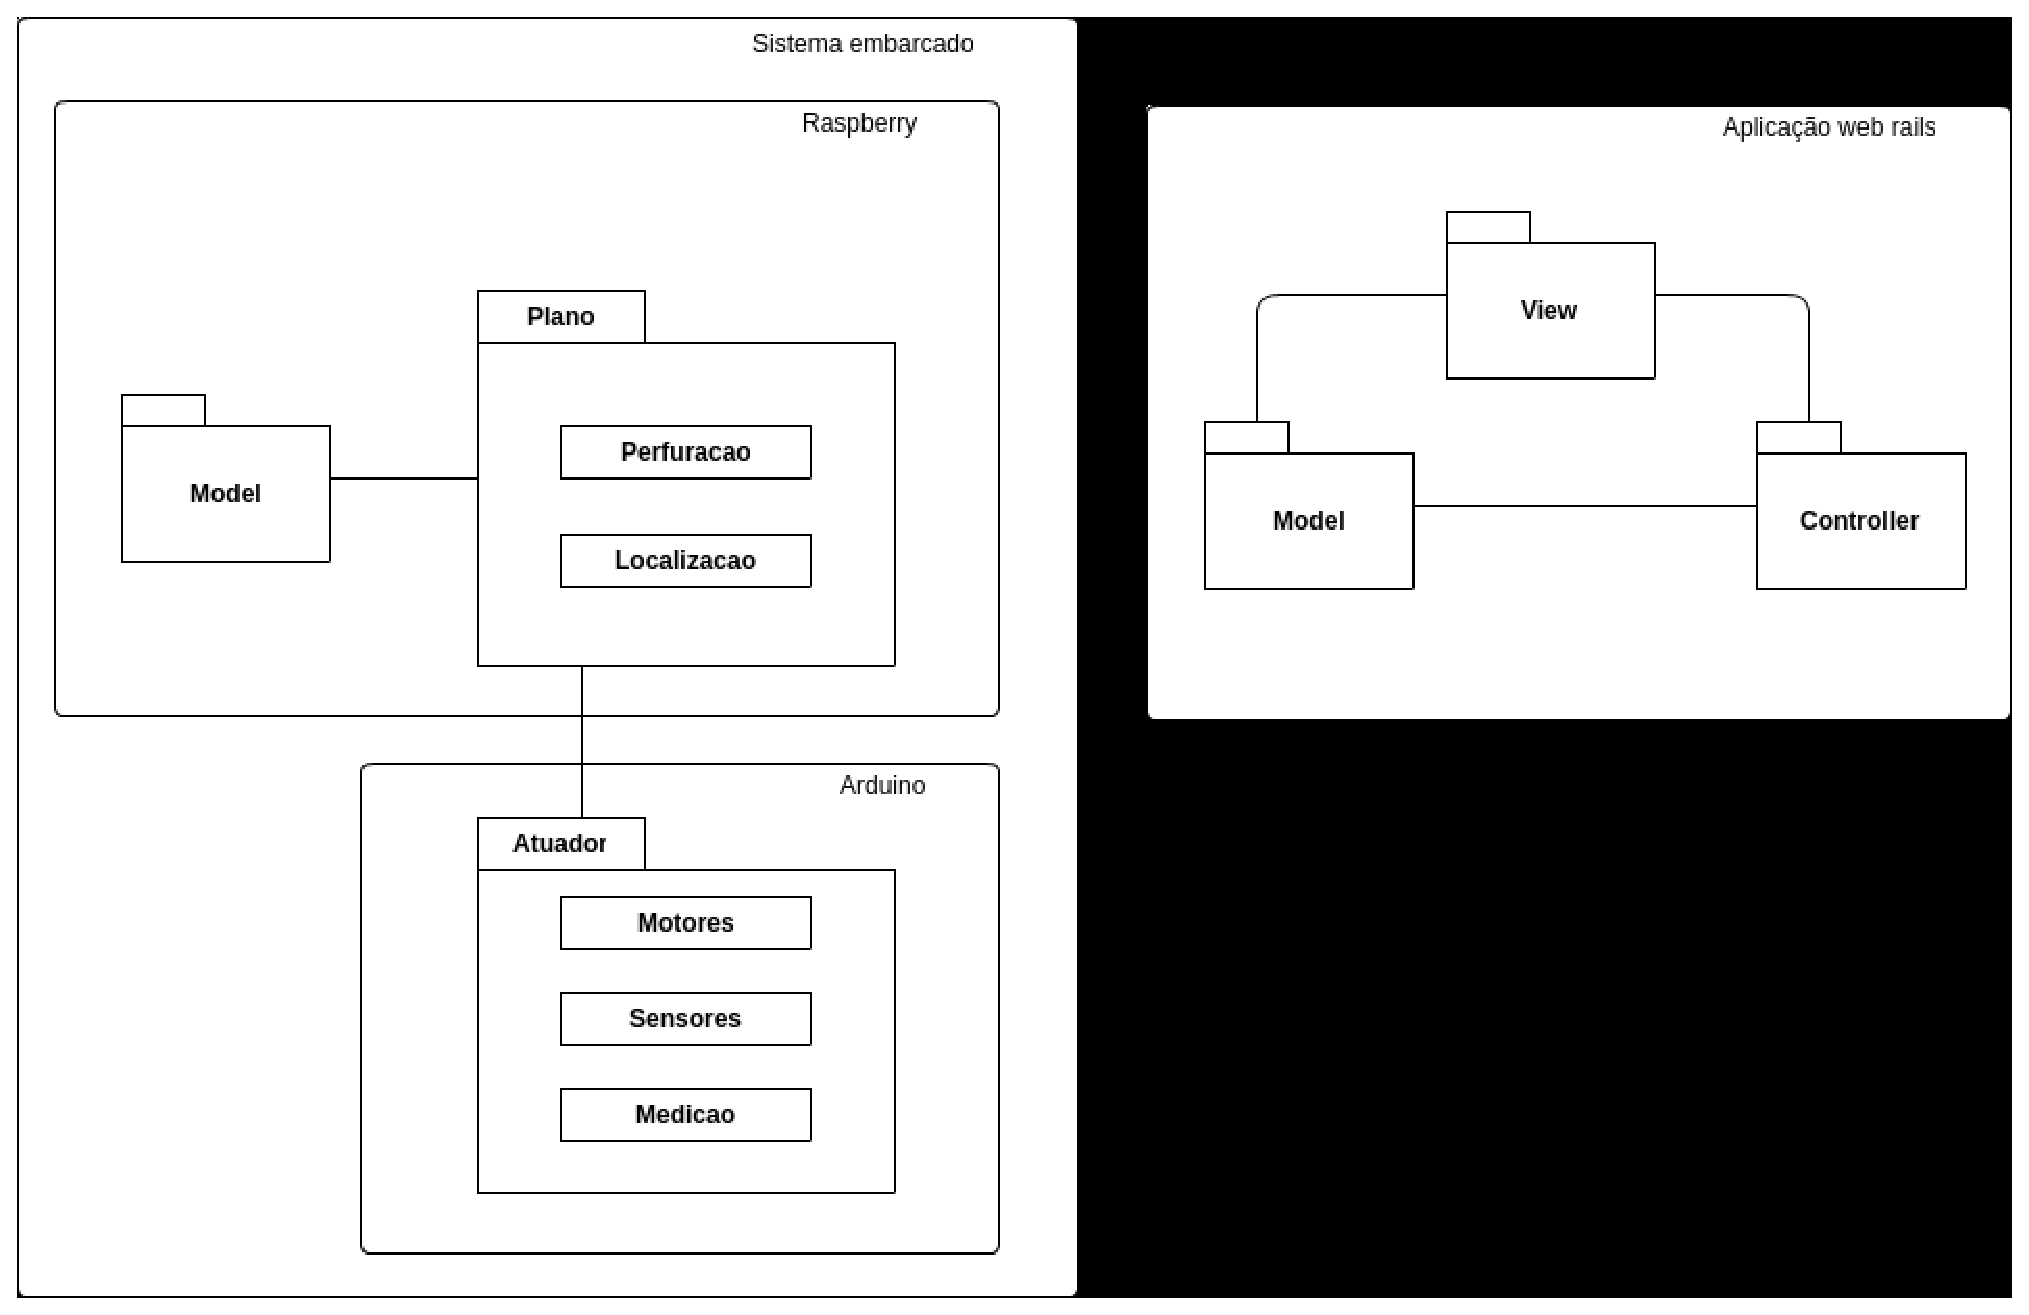
\includegraphics[width=.8\textwidth]{figuras/Arquitetura.eps}
		\caption{\label{fig:arquitetura_sistema}Arquitetura do sistema.}
	\end{center}
\end{figure}